\documentclass[t,usenames,dvipsnames]{beamer}
\usetheme{Copenhagen}
\setbeamertemplate{headline}{} % remove toc from headers
\beamertemplatenavigationsymbolsempty

\usepackage{amsmath, tikz, xcolor, bm}
\usetikzlibrary{arrows, calc, decorations.pathreplacing, patterns}

\title{Ellipses}
\author{}
\date{}

\AtBeginSection[]
{
  \begin{frame}
    \frametitle{Objectives}
    \tableofcontents[currentsection]
  \end{frame}
}

\begin{document}

\begin{frame}
    \titlepage
\end{frame}

\section{Identify the center, vertices, and foci of an ellipse.}

\begin{frame}{Intro}
An \alert{ellipse} is the set of points such that the sum of their distances from 2 fixed points (called \alert{foci}) is constant. \newline\\  \pause
\begin{center}
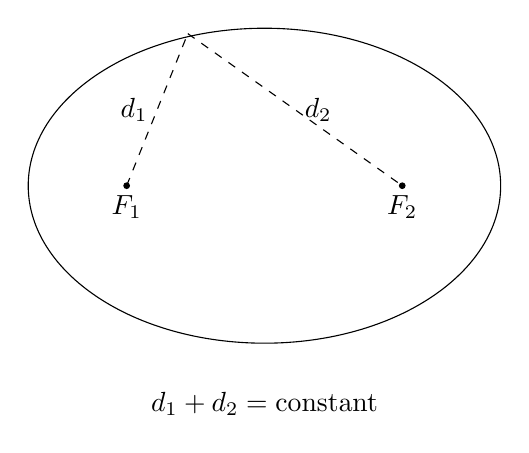
\begin{tikzpicture}
    \draw (0,0) ellipse (3cm and 2cm);
    \coordinate (A) at (-1.75,0);
    \coordinate (C) at (1.75,0);
    \coordinate (B) at ($(A) + (75:3 and 2)$);
    \draw [fill=black] (A) circle (1pt) node [below] {$F_1$};
    \draw [fill=black] (C) circle (1pt) node [below] {$F_2$};
    \draw [dashed] (A) -- node [midway, left] {$d_1$} (B);
    \draw [dashed] (B) -- node [midway, right] {$d_2$} (C);
    \node at (0,-2.5) [below] {$d_1+d_2=\text{constant}$};
\end{tikzpicture}
\end{center}
\end{frame}

\begin{frame}{Intro}
Ellipses will typically either appear wider or taller based on their equation.  \newline\\  \pause
\begin{center}
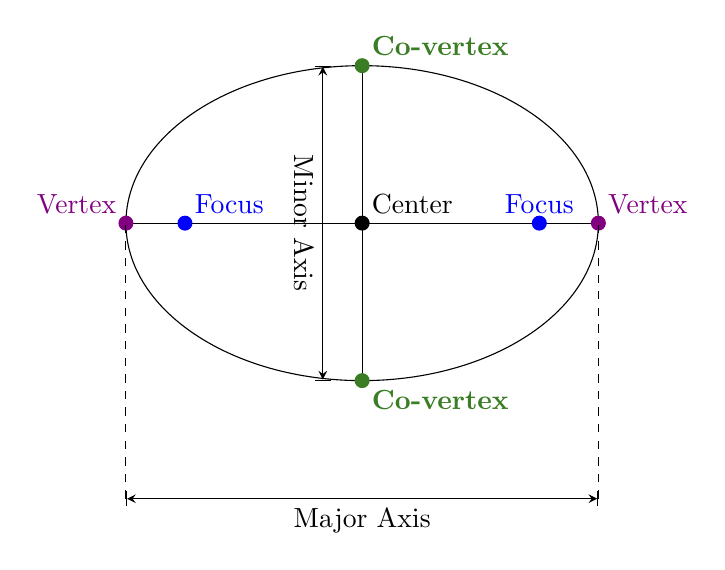
\begin{tikzpicture}
    \draw [] (-3,0) -- (3,0);
    \draw [] (0,-2) -- (0,2);
    \draw (0,0) ellipse (3cm and 2cm);
    \draw [fill=black] (0,0) circle (2.5pt);
    \node at (0,0) [anchor=south west] {Center};
    \draw [color=violet, fill=violet] (3,0) circle (2.5pt);
    \node at (3,0) [anchor=south west, color=violet] {Vertex};
    \draw [color=violet, fill=violet] (-3,0) circle (2.5pt);
    \node at (-3,0) [anchor=south east, color=violet] {Vertex};
    \draw [fill=blue, color=blue] (-2.25,0) circle (2.5pt);
    \node at (-2.25,0) [anchor=south west] {\color{blue}Focus};
    \draw [fill=blue, color=blue] (2.25,0) circle (2.5pt);
    \node at (2.25,0) [anchor=south] {\color{blue}Focus};
    \draw [color=OliveGreen, fill=OliveGreen] (0,2) circle (2.5pt);
    \node at (0,2.25) [anchor=south west, color=OliveGreen, yshift=-0.25cm] {\textbf{Co-vertex}};
    \draw [color=OliveGreen, fill=OliveGreen] (0,-2) circle (2.5pt);
    \node at (0,-2.25) [anchor=north west, color=OliveGreen, yshift=0.25cm] {\textbf{Co-vertex}};
    \draw [|<->|, >=stealth] (-3,-3.5) -- (3,-3.5);
    \draw [dashed] (-3,-3.5) -- (-3,0); 
    \draw [dashed] (3,-3.5) -- (3,0);
    \node at (0,-3.5) [anchor=north] {Major Axis};
    \draw [|<->|, >=stealth] (-0.5,-2) -- (-0.5,2);
    \node at (-0.5,0) [rotate=270, anchor=north] {Minor Axis};
\end{tikzpicture}
\end{center}
\end{frame}

\begin{frame}{Intro}
\begin{center}
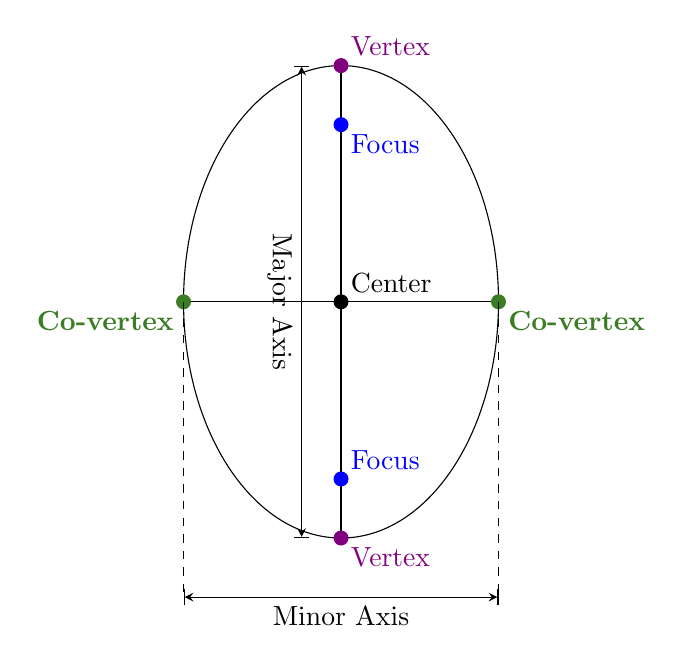
\begin{tikzpicture}
    \draw (-2,0) -- (2,0);
    \draw (0,-3) -- (0,3);
    \draw (0,0) ellipse (2cm and 3cm);
    \draw [fill=black] (0,0) circle (2.5pt);
    \node at (0,0) [anchor=south west] {Center};
    \draw [color=violet, fill=violet] (0,3) circle (2.5pt);
    \node at (0,3) [anchor=south west, color=violet] {Vertex};
    \draw [color=violet, fill=violet] (0,-3) circle (2.5pt);
    \node at (0,-3) [anchor=north west, color=violet] {Vertex};
    \draw [fill=blue, color=blue] (0,-2.25) circle (2.5pt);
    \node at (0,-2.25) [anchor=south west] {\color{blue}Focus};
    \draw [fill=blue, color=blue] (0,2.25) circle (2.5pt);
    \node at (0,2.25) [anchor=north west] {\color{blue}Focus};
    \draw [color=OliveGreen, fill=OliveGreen] (2,0) circle (2.5pt);
    \node at (2,0) [anchor=north west, color=OliveGreen] {\textbf{Co-vertex}};
    \draw [color=OliveGreen, fill=OliveGreen] (-2,0) circle (2.5pt);
    \node at (-2,0) [anchor=north east, color=OliveGreen] {\textbf{Co-vertex}};
    \draw [|<->|, >=stealth] (-0.5,3) -- (-0.5,-3);
    \node at (-0.5,0) [rotate=270, anchor=north] {Major Axis};
    \draw [|<->|, >=stealth] (-2,-3.75) -- (2,-3.75);
    \node at (0,-3.75) [anchor=north] {Minor Axis};
    \draw [dashed] (-2,0) -- (-2,-3.75);
    \draw [dashed] (2,0) -- (2,-3.75);    
\end{tikzpicture}
\end{center}
\end{frame}

\begin{frame}{Intro}
The \alert{center} of an ellipse is denoted by $(h, k)$, just like with circles.    \newline\\ \pause

Each focal point (\textit{pl: foci}) is $c$ units from the center. The foci are on the \alert{major axis}.  \newline\\  \pause
Each vertex (\textit{pl: vertices}) also lies on the major axis, and is $a$ units away from the center. \newline\\  \pause
Each \alert{co-vertex} (\textit{pl: co-vertices}) lies on the \alert{minor axis}, which is perpendicular to the major axis. The co-vertices are each $b$ units away from the center. 
\end{frame}

\begin{frame}{Intro}
\begin{center}
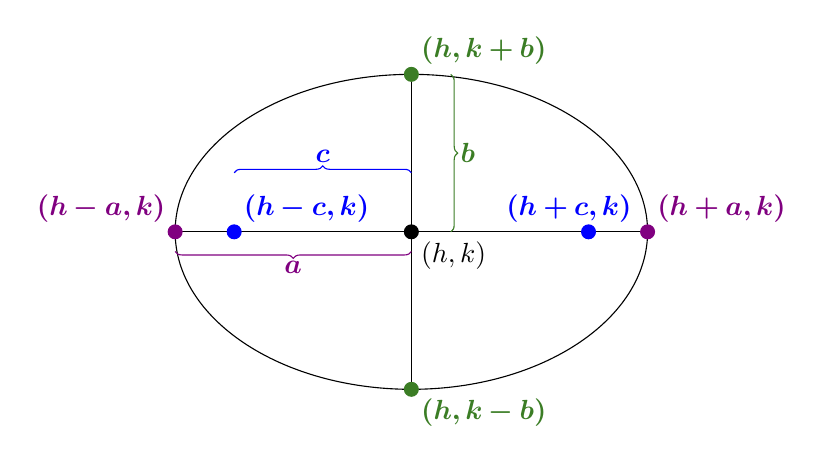
\begin{tikzpicture}
    \draw [] (-3,0) -- (3,0);
    \draw [] (0,-2) -- (0,2);
    \draw (0,0) ellipse (3cm and 2cm);
    \draw [fill=black] (0,0) circle (2.5pt);
    \node at (0,0) [anchor=north west] {$(h,k)$};
    \draw [color=violet, fill=violet] (3,0) circle (2.5pt);
    \node at (3,0) [anchor=south west, color=violet] {$\bm{(h+a,k)}$};
    \draw [color=violet, fill=violet] (-3,0) circle (2.5pt);
    \node at (-3,0) [anchor=south east, color=violet] {$\bm{(h-a,k)}$};
    \draw [fill=blue, color=blue] (-2.25,0) circle (2.5pt);
    \node at (-2.25,0) [anchor=south west] {\color{blue}$\bm{(h-c,k)}$};
    \draw [fill=blue, color=blue] (2.25,0) circle (2.5pt);
    \node at (2.25,0) [anchor=south, xshift=-0.25cm] {\color{blue}$\bm{(h+c,k)}$};
    \draw [color=OliveGreen, fill=OliveGreen] (0,2) circle (2.5pt);
    \node at (0,2.25) [anchor=south west, color=OliveGreen, yshift=-0.25cm] {$\bm{(h,k+b)}$};
    \draw [color=OliveGreen, fill=OliveGreen] (0,-2) circle (2.5pt);
    \node at (0,-2.25) [anchor=north west, color=OliveGreen, yshift=0.25cm] {$\bm{(h, k-b)}$};
    \draw [decoration={brace}, decorate, color=violet, yshift=-0.25cm] (0,0) -- (-3,0);
    \node at (-1.5,-0.25) [anchor=north, color=violet] {$\bm{a}$};
    \draw [decoration={brace}, decorate, color=OliveGreen, xshift=0.5cm] (0,2) -- (0,0);
    \node at (0.5,1) [anchor=west, color=OliveGreen] {$\bm{b}$};
    \draw [decoration={brace}, decorate, color=blue, yshift=0.75cm] (-2.25,0) -- (0,0);
    \node at (-1.125,0.75) [anchor=south, color=blue] {$\bm{c}$};
\end{tikzpicture}
\\[10pt]  \pause
$\dfrac{(x-h)^2}{a^2} + \dfrac{(y-k)^2}{b^2} = 1$
\end{center}
\end{frame}

\begin{frame}{Intro}
\begin{center}
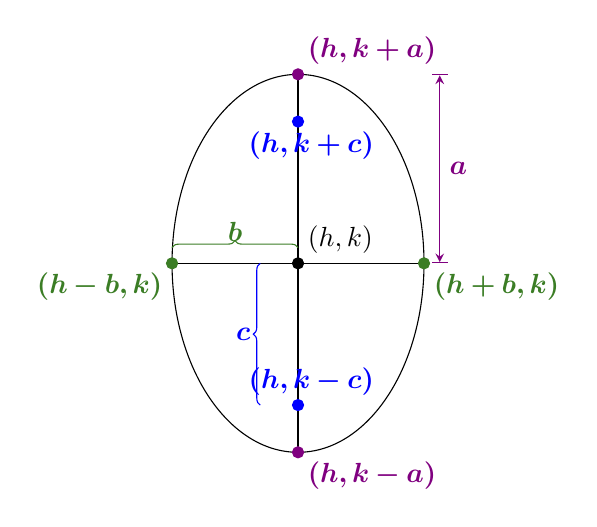
\begin{tikzpicture}[scale=0.8]
    \draw (-2,0) -- (2,0);
    \draw (0,-3) -- (0,3);
    \draw (0,0) ellipse (2cm and 3cm);
    \draw [fill=black] (0,0) circle (2.5pt);
    \node at (0,0) [anchor=south west] {$(h, k)$};
    \draw [color=violet, fill=violet] (0,3) circle (2.5pt);
    \node at (0,3) [anchor=south west, color=violet] {$\bm{(h, k+a)}$};
    \draw [color=violet, fill=violet] (0,-3) circle (2.5pt);
    \node at (0,-3) [anchor=north west, color=violet] {$\bm{(h, k-a)}$};
    \draw [fill=blue, color=blue] (0,-2.25) circle (2.5pt);
    \node at (0,-2.25) [anchor=south west, xshift=-0.75cm] {\color{blue}$\bm{(h, k-c)}$};
    \draw [fill=blue, color=blue] (0,2.25) circle (2.5pt);
    \node at (0,2.25) [anchor=north west, xshift=-0.75cm] {\color{blue}$\bm{(h, k+c)}$};
    \draw [color=OliveGreen, fill=OliveGreen] (2,0) circle (2.5pt);
    \node at (2,0) [anchor=north west, color=OliveGreen] {$\bm{(h+b,k)}$};
    \draw [color=OliveGreen, fill=OliveGreen] (-2,0) circle (2.5pt);
    \node at (-2,0) [anchor=north east, color=OliveGreen] {$\bm{(h-b,k)}$};
    \draw [decoration={brace}, decorate, yshift=0.25cm, color=OliveGreen] (-2,0) -- (0,0);
    \node at (-1,0.5) [color=OliveGreen] {$\bm{b}$};
    \draw [decoration={brace}, decorate, color=blue, xshift=-0.6cm] (0,-2.25) -- (0,0);
    \node at (-0.6, -1.125) [anchor=east, color=blue] {$\bm{c}$};
    \draw [|<->|, >=stealth, color=violet] (2.25,0) -- (2.25,3);
    \node at (2.25, 1.5) [anchor=west, color=violet] {$\bm{a}$};
\end{tikzpicture}   \pause
$\dfrac{(y-k)^2}{a^2} + \dfrac{(x-h)^2}{b^2} = 1$
\end{center}
\end{frame}

\begin{frame}{Intro}
\emph{Note:} In both cases, $c^2 = a^2 - b^2$, and $a > b$.    
\end{frame}

\begin{frame}{Example 1}
Find the center, the lines containing the major and minor axes, the vertices, the endpoints of the minor axis (co-vertices), and the foci for
\[
\frac{(x+1)^2}{9} + \frac{(y-2)^2}{25} = 1
\]
\end{frame}
\begin{frame}{Example 1 $\frac{(x+1)^2}{9} + \frac{(y-2)^2}{25} = 1$}
\begin{minipage}{0.4\textwidth}
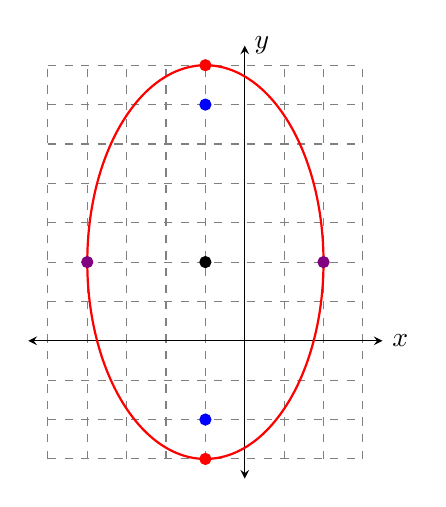
\begin{tikzpicture}[scale=0.5]
\draw[dashed, gray] (-5,-3) grid (3,7);
\draw[<->,>=stealth] (-5.5,0) -- (3.5,0) node [right] {$x$};
\draw[<->,>=stealth] (0,-3.5) -- (0,7.5) node [right] {$y$};
\draw[color=red, thick] (-1,2) ellipse (3cm and 5cm);
\onslide<2->{\draw[fill=black] (-1,2) circle (4pt);}
\onslide<5->{
\draw[color=red,fill=red] (-1,7) circle (4pt);
\draw[color=red,fill=red] (-1,-3) circle (4pt);}
\onslide<9->{
\draw[color=violet,fill=violet] (-4,2) circle (4pt);
\draw[color=violet,fill=violet] (2,2) circle (4pt);}
\onslide<13->{
\draw[color=blue,fill=blue] (-1,6) circle (4pt);
\draw[color=blue,fill=blue] (-1,-2) circle (4pt);}
\end{tikzpicture}
\end{minipage}
\hspace{0.5cm}
\begin{minipage}{0.5\textwidth}
\onslide<2->{Center: $(-1,2)$} \\[8pt]
{\color{red}
\onslide<3->{Vertices: $a^2 = 25 \longrightarrow a = \pm 5$} \\
\onslide<4->{Vertices: $(-1,2\pm 5)$} \\
\onslide<5->{Vertices: $(-1,7)\text{ and } (-1,-3)$}} \\[8pt]
\onslide<6->{Major Axis Line: $x = -1$} \\[8pt]
{\color{violet}
\onslide<7->{Co-Vertices: $b^2 = 9 \longrightarrow b = \pm 3$} \\
\onslide<8->{Co-Vertices: $(-1 \pm 3, 2)$} \\
\onslide<9->{Co-Vertices: $(-4,2) \text{ and } (2,2)$}} \\[8pt]
\onslide<10->{Minor Axis Line: $y = 2$} \\[8pt]
{\color{blue}
\onslide<11->{Foci: $c^2 = 25 - 9 \longrightarrow c = \pm 4$} \\
\onslide<12->{Foci: $(-1,2\pm4)$} \\
\onslide<13->{Foci: $(-1,-2) \text{ and } (-1,6)$}}
\end{minipage}
\end{frame}


\section{Write the equation of an ellipse in standard form.}

\begin{frame}{Example 2}
Find the equation of the ellipse with foci $(2, 1)$ and $(4, 1)$ and vertex $(0, 1)$.   \newline\\
\begin{minipage}{0.4\textwidth}
\onslide<2->{
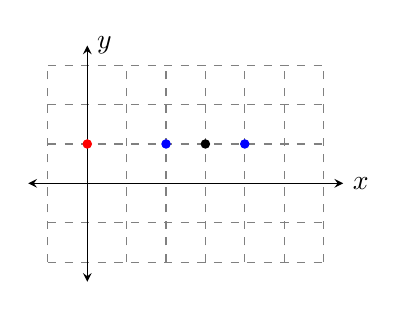
\begin{tikzpicture}[scale=0.5]
\draw[dashed, gray] (-1,-2) grid (6,3);
\draw[<->,>=stealth] (-1.5,0) -- (6.5,0) node [right] {$x$};
\draw[<->,>=stealth] (0,-2.5) -- (0,3.5) node [right] {$y$};
\draw[color=blue,fill=blue] (2,1) circle (3pt);
\draw[color=blue,fill=blue] (4,1) circle (3pt);
\draw[color=red,fill=red] (0,1) circle (3pt);
\onslide<3->{\draw[fill=black] (3,1) circle (3pt);}
\end{tikzpicture}}
\end{minipage}
\hspace{0.25cm}
\begin{minipage}{0.5\textwidth}
\onslide<3->{Center: $\left(\dfrac{2+4}{2}, \dfrac{1+1}{2}\right)$ = $(3,1)$} \\[8pt]
\onslide<4->{$c = 1, \quad a = 3$}
\begin{align*}
    \onslide<5->{3^2 - b^2 &= 1^2} \\
    \onslide<6->{9 - b^2 &= 1} \\
    \onslide<7->{-b^2 &= -8} \\
    \onslide<8->{b^2 &= 8} 
\end{align*}
\[
\onslide<9->{\frac{(x-3)^2}{9} + \frac{(y-1)^2}{8} = 1}
\]
\end{minipage}
\end{frame}

\begin{frame}{Writing the Equation of an Ellipse}
    Writing the equation of an ellipse in standard form is a lot like that for circles.
\end{frame}

\begin{frame}{Example 3}
Find the center, the lines containing the major and minor axes, the vertices, the endpoints of the minor axis, and the foci for $x^2 -2x + 4y^2 + 24y + 33 = 0$  
\begin{align*}
    \onslide<2->{{\color{red}x^2 -2x} + {\color{blue}4y^2 + 24y} &= -33} \\[8pt]
    \onslide<3->{{\color{red}\text{Vertex: } (1,-1)} \quad &  {\color{blue}\text{Vertex: } (-3,-36)}} \\[8pt]
    \onslide<4->{(x-1)^2 + 4(y+3)^2 &= -33 + |{\color{red}-1}| + |{\color{blue}-36}|} \\[8pt]
    \onslide<5->{(x-1)^2 + 4(y+3)^2 &= 4} \\[8pt]
    \onslide<6->{\frac{(x-1)^2}{4} + \frac{(y+3)^2}{1} &= 1}
\end{align*}
\end{frame}

\begin{frame}{Example 3 $\frac{(x-1)^2}{4} + \frac{(y+3)^2}{1} = 1$}
    Center: $(1,-3)$
    \begin{align*}
        \onslide<2->{a^2 &= 4} \\
        \onslide<3->{a &= \pm 2} \\
    \end{align*}
    \onslide<4->{Vertices: $(1\pm 2,-3)$} \\[8pt]
    \onslide<5->{Vertices: $(-1,-3) \text{ and } (3,-3)$} \\[8pt]
    \onslide<6->{Major axis: $y = -3$} \\
\end{frame}
\begin{frame}{Example 3}
    Co-Vertices: $b^2 = 1 \longrightarrow b = \pm 1$    \\[8pt]
    \onslide<2->{Co-Vertices: $(1,-3\pm 1) \longrightarrow (1,-4) \text{ and } (1,-2)$} \\[8pt]
    \onslide<3->{Minor axis: $x = 1$} \\[8pt]
    
    \onslide<4->{Foci:}
    \begin{align*}
        \onslide<5->{c^2 &= 4 - 1} \\
        \onslide<6->{c &= \pm \sqrt{3} }
    \end{align*}
    \onslide<7->{Foci: $(1 \pm \sqrt{3}, -3)$}
\end{frame}

\begin{frame}{Eccentricity}
The ``roundness" of an ellipse is measured by its \alert{eccentricity}. It is a ratio and is denoted by $e$.  \newline\\
\[
e = \dfrac{\text{Distance from center to focus}}{\text{Distance from center to vertex}} \onslide<2->{= \dfrac{c}{a}}
\]
\end{frame}

\begin{frame}{Example 4}
Find the equation of the ellipse with vertices $(\pm 5, 0)$ and eccentricity $e = \frac{1}{4}$.  \newline\\
\onslide<2->{Center: $(0,0)$}
\begin{align*}
    \onslide<3->{\frac{1}{4} &= \frac{c}{a}} \\[8pt]
    \onslide<4->{\frac{1}{4} &= \frac{c}{5}} \\[8pt]
    \onslide<5->{4c &= 5} \\[8pt]
    \onslide<6->{c &= \frac{5}{4}} 
\end{align*}
\end{frame}

\begin{frame}{Example 4 \quad $a = 5, c = \frac{5}{4}$}
    \begin{align*}
        \left(\frac{5}{4}\right)^2 &= 5^2 - b^2 \\[10pt]
        \frac{25}{16} &= 25 - b^2 \\[10pt]
        -\frac{375}{16} &= -b^2 \\[10pt]
        b^2 &= \frac{375}{16} \\
    \end{align*}
\end{frame}

\begin{frame}{Example 4}
    \begin{align*}
        \frac{x^2}{25} + \frac{y^2}{\frac{375}{16}} &= 1 \\[10pt]
        \onslide<2->{\frac{x^2}{25} + \frac{y^2}{\frac{375}{16}}{\color{blue}\left(\frac{16}{16}\right)} &= 1} \\[10pt]
        \onslide<3->{\frac{x^2}{25} + \frac{16y^2}{375} &= 1}
    \end{align*}
\end{frame}

\section{Solve application problems involving ellipses.}

\begin{frame}{Example 5}
Jamie and Jason want to exchange secrets (terrible secrets) from across a crowded whispering gallery. A whispering gallery is a room which, in cross section, is half of an ellipse.  If the room is 40 feet high at the center and 100 feet wide at the floor, how far from the outer wall should each of them stand so that they will be positioned at the foci of the ellipse?  \newline\\  \pause

\begin{center}
\begin{tikzpicture}[scale=0.6]
\draw[<->,>=stealth] (-5.5,0) -- (5.5,0);
\draw[->,>=stealth] (0,0) -- (0,4.5);
\draw[color=red,fill=red] (5,0) circle (3pt);
\draw[color=violet,fill=violet] (0,4) circle (3pt);
\draw[color=blue,fill=blue] (3,0) circle (3pt);
\draw [decoration={brace}, decorate, color=red, yshift=-0.25cm] (5,0) -- (0,0) node [midway, below] {\scriptsize $a=50$}; 
\draw [decoration={brace}, decorate, color=violet, xshift=-0.25cm] (0,0) -- (0,4) node [midway,left] {\scriptsize $b=40$};
\draw [decoration={brace}, decorate, color=blue, yshift=0.25cm] (0,0) -- (3,0) node [midway, above] {\scriptsize $c=?$};
\end{tikzpicture}
\end{center}
\end{frame}

\begin{frame}{Example 5}
\begin{center}
\begin{tikzpicture}[scale=0.6]
\draw[<->,>=stealth] (-5.5,0) -- (5.5,0);
\draw[->,>=stealth] (0,0) -- (0,4.5);
\draw[color=red,fill=red] (5,0) circle (3pt);
\draw[color=violet,fill=violet] (0,4) circle (3pt);
\draw[color=blue,fill=blue] (3,0) circle (3pt);
\draw [decoration={brace}, decorate, color=red, yshift=-0.25cm] (5,0) -- (0,0) node [midway, below] {\scriptsize $a=50$}; 
\draw [decoration={brace}, decorate, color=violet, xshift=-0.25cm] (0,0) -- (0,4) node [midway,left] {\scriptsize $b=40$};
\draw [decoration={brace}, decorate, color=blue, yshift=0.25cm] (0,0) -- (3,0) node [midway, above] {\scriptsize $c=?$};
\end{tikzpicture}
\end{center}
\begin{align*}
    \onslide<2->{c^2 &= 50^2 - 40^2} \\[8pt]
    \onslide<3->{c^2 &= 900} \\[8pt]
    \onslide<4->{c &= \sqrt{900}} \\[8pt]
    \onslide<5->{c &= 30\text{ feet}}
\end{align*}
\end{frame}

\end{document}
